\section{Wichtige Formeln}
	
	\renewcommand{\arraystretch}{2.1}
	\begin{tabular}[c]{ | p{5.1cm} | p{5.4cm} | l | }
		\hline
		\textbf{Explixit (Kartesisch)} & \textbf{Parameter} & \textbf{Polar} \\
		\hline
		\multicolumn{3}{| l |}{\textbf{Anstieg einer Kurve} \formelbuch{????} \quad \textit{1.Ableitung, 2. Ableitung} \qquad \textit{Anstieg in $P_0$ $\in$ C}} \\
    	\hline   
    	$m=y'=f'(x_o) \qquad y'' = f''(x_0)$ & 
    	$m=y'=\frac{\dot{y}}{\dot{x}} \qquad 
    	y'' = \frac{\dot{x} \ddot{y} - \dot{y}\ddot{x}}{\dot{x}^3}$ &
    	$m=y'=\frac{r'(\varphi) \sin(\varphi) + r(\varphi) \cdot
    	\cos(\varphi)}{r'(\varphi) \cos(\varphi)-r(\varphi) \cdot \sin(\varphi)}$
    	\\
		
		\hline
		\multicolumn{3}{| l |}{\textbf{Bogenlänge} \formelbuch{514} \qquad\textit{zwischen $P_1$,$P_2$ $\in$ C}} \\ %Seitenzahlen OK 10 Auflage
    	\hline
    	$s=\int\limits_a^b{\sqrt{1+(f'(x))^2}dx}$ & 
    	$|s|=\int\limits_{t_1}^{t_2}{\sqrt{\dot{x}^2(t)+\dot{y}^2(t)}dt}$ &
		$|s|=\int\limits_{\varphi_1}^{\varphi_2}{\sqrt{(r'(\varphi))^2+(r(\varphi))^2}d\varphi}$\\
		
		\hline		
		\multicolumn{3}{| l |}{\textbf{Krümmung ebener Kurven} {\formelbuch{253ff}} \qquad \qquad $\frac{\Delta\alpha}{\Delta s}$ %Seitenzahlen OK 10 Auflage
			$\quad$ Scheitel bei: $K'(x)=0 \quad$ \textit{und} $\quad K''(x)\neq 0
			\begin{cases}
			K(x)<0 & \text{Maxima}\\
			K(x)>0 & \text{Minima}
			\end{cases}$}\\%
		%
    	\hline
       	$\kappa=\frac{f''(x)}{\left(\sqrt{1+(f'(x))^2}\right)^3}$ &
    	$\kappa=\frac{\dot{x}(t)\ddot{y}(t)-\dot{y}(t)\ddot{x}(t)}{\left(\sqrt{(\dot{x}(t))^2+(\dot{y}(t))^2}\right)^3}$ &
		$\kappa=\frac{2(r'(\varphi))^2-r(\varphi)r''(\varphi)+(r(\varphi))^2}{\left(\sqrt{(r'(\varphi))^2+(r(\varphi))^2}\right)^3}$\\   	
		
		\hline
		\multicolumn{3}{| l |}{Konvex (Linkskurve): $\kappa \geq 0 \qquad$ Streng
		konvex: $\kappa > 0 \qquad$ Wendepunkt: $\kappa = 0 \qquad$ Analog für konkav}\\
		
		\hline
		\multicolumn{3}{| l |}{\textbf{Krümmungskreisradius} {\formelbuch{254}} \qquad $r = |\frac{1}{\kappa}|$} \\ %Seitenzahlen OK 10 Auflage
		\hline%
		$r = \left|\frac{\left(\sqrt{1+(f'(x))^2}\right)^3}{f''(x)} \right|$ &
		$r = \left|\frac{\left(\sqrt{(\dot{x}(t))^2+(\dot{y}(t))^2}\right)^3}
		{\dot{x}(t)\ddot{y}(t)-\dot{y}(t)\ddot{x}(t)} \right|$ & 
		$r = \left|\frac{\left((\sqrt{(r'(\varphi))^2+(r(\varphi))^2}\right)^3}
		{2(r'(\varphi))^2-r(\varphi)r''(\varphi)+(r(\varphi))^2} \right|$ \\%
		%
		\hline		
		\multicolumn{3}{| l |}{\textbf{Flächeninhalt} {\formelbuch{514}} \quad \textit{um x-Achse} \qquad\qquad \textit{ $\quad$ y-Achse: Umkerhfunktion $f^{-1}(x)$ von $y_{0}$ bis $y_{1}$ integrieren}}\\ %Seitenzahlen OK 10 Auflage
    	\hline
    	$A=\int\limits_a^b{f(x)}dx$  & 
    	$A=\frac{1}{2}\int\limits_{t_1}^{t_2}{[x(t)\dot{y}(t)-\dot{x}(t)y(t)]dt}$ &
		$A=\frac{1}{2}\int\limits_{\varphi_1}^{\varphi_2}{(r(\varphi))^2d\varphi}$\\  
    	
		\hline		
		\multicolumn{3}{| l |}{\textbf{Volumen} {\formelbuch{515}} \quad \textit{mit Meridian C (Rotationskörper)}} \\ %Seitenzahlen OK 10 Auflage
    	\hline
		$V=\pi\int\limits_a^b(f(x))^2dx$ & 
    	$V=\pi\left|\int\limits_{t_1}^{t_2}{(y(t))^2\dot{x}(t)dt}\right|$ &
		$V=\pi\left|\int\limits_{\varphi_1}^{\varphi_2}{r^2(\varphi)\sin^2\varphi[r'(\varphi)\cos(\varphi)-r(\varphi)\sin(\varphi)]d\varphi}\right|$\\  
    	
		\hline		
		\multicolumn{3}{| l |}{\textbf{Oberflächeninhalt} {\formelbuch{515}} \quad \textit{mit Meridian C (Rotationskörper)}} \\ %Seitenzahlen OK 10 Auflage
    	\hline
   		$O=2\pi\int\limits_a^b{|f(x)|\sqrt{1+(f'(x))^2}dx}$ & 
    	$O=2\pi\int\limits_{t_1}^{t_2}{|y(t)|\sqrt{\dot{x}^2(t)+(\dot{y}^2(t))}dt}$ &
		$O=2\pi\int\limits_{\varphi_1}^{\varphi_2}{|r(\varphi)\sin\varphi|\sqrt{(r'(\varphi))^2+(r(\varphi))^2}d\varphi}$\\  
    	\hline
   	    \multicolumn{3}{| l |}{
   		Polar: $\quad \sin \varphi=$ Drehung um Polgerade \qquad $\cos y=$ Drehung um y-Achse $\left(f=\frac{\pi}{2}\right) \quad \rightarrow$ siehe Fläche
    	}\\
    	\hline
	\end{tabular}
	
	\subsection{Evolute (Kurve des Krümmungskreis-Zentrums) {\formelbuch{262}}} %Seitenzahlen OK 10 Auflage
		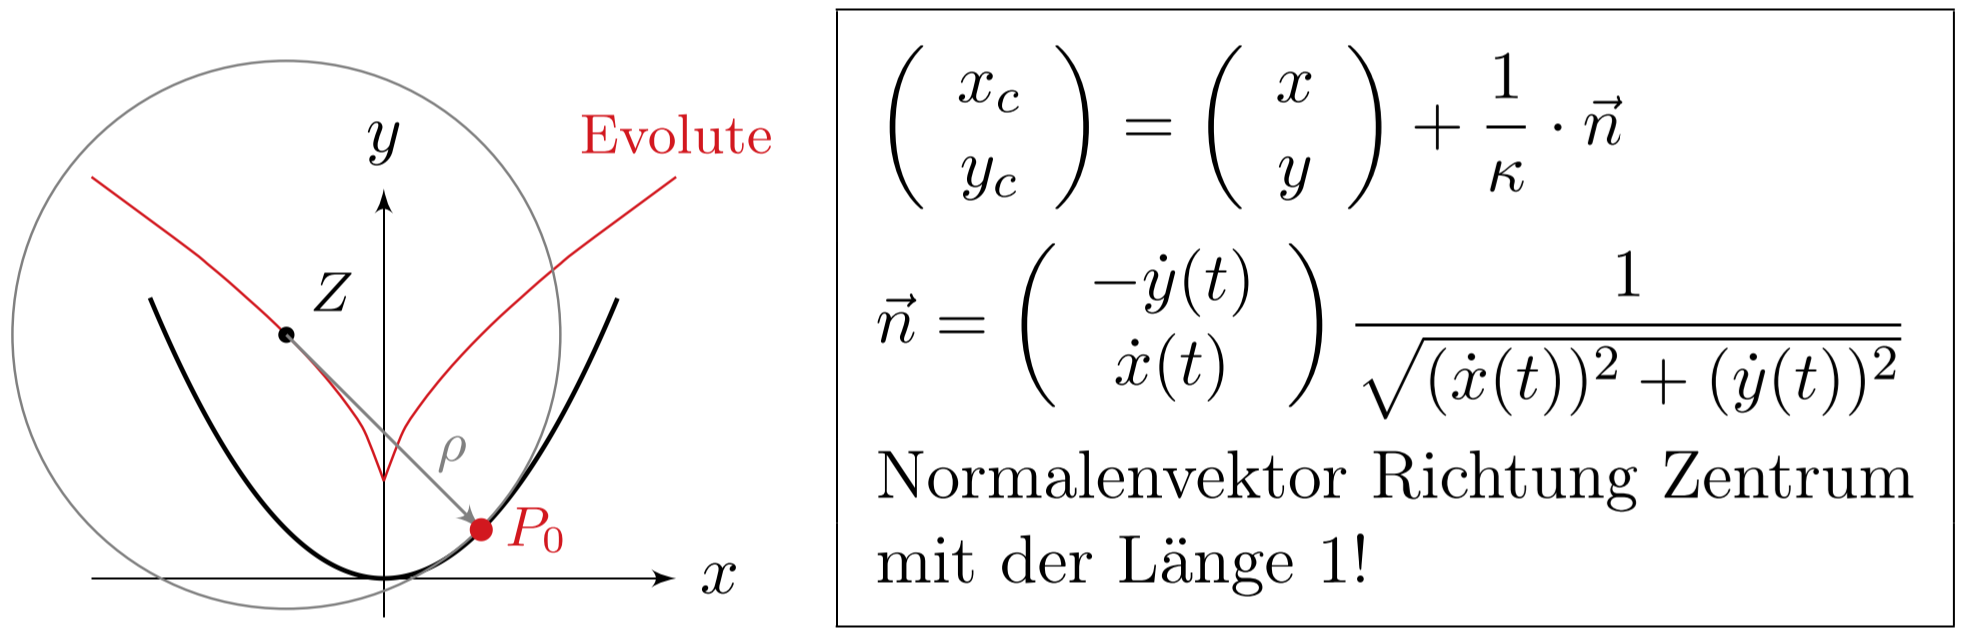
\includegraphics[width=.5\textwidth]{bilder/evolute_zeichnung.png}\\
			\begin{tabular}[c]{| p{4.4cm} | p{5.4cm} | l | }
				\hline
		    	\multicolumn{3}{| l |}{\textbf{Krümmungskreismittelpunkt} {\formelbuch{255}}} \\ %Seitenzahlen OK 10 Auflage
				\hline
				\textbf{Explixit (Kartesisch)} & \textbf{Parameter} & \textbf{Polar} \\
				\hline
				$x_{c}=x-\frac{y^{\prime}\left(1+y^{\prime 2}\right)}{y^{\prime \prime}}$ & $x_{c}(t)=x(t)-\dot{y}(t) \frac{(\dot{x}(t))^{2}+(\dot{y}(t))^{2}}{\dot{x}(t) \ddot{y}(t)-\ddot{x}(t) \dot{y}(t)}$ & $x_{c}=r(\varphi) \cos (\varphi)-\frac{\left[(r(\varphi))^{2}+\left(r^{\prime}(\varphi)\right)^{2}\right] \cdot\left[r(\varphi) \cos (\varphi)+r^{\prime}(\varphi) \sin (\varphi)\right]}{(r(\varphi))^{2}+2\left(r^{\prime}(\varphi)\right)^{2}-r(\varphi) r^{\prime \prime}(\varphi)}$
				\\[1mm]
				$y_{c}=y+\frac{1+y^{\prime 2}}{y^{\prime \prime}}$ & $y_{c}(t)=y(t)+\dot{x}(t) \frac{(\dot{x}(t))^{2}+(\dot{y}(t))^{2}}{\dot{x}(t) \ddot{y}(t)-\ddot{x}(t) \dot{y}(t)}$ & $y_{c}=r(\varphi) \sin (\varphi)-\frac{\left[(r(\varphi))^{2}+\left(r^{\prime}(\varphi)\right)^{2}\right] \cdot\left[r(\varphi) \sin (\varphi)-r^{\prime}(\varphi) \cos (\varphi)\right]}{(r(\varphi))^{2}+2\left(r^{\prime}(\varphi)\right)^{2}-r(\varphi) r^{\prime \prime}(\varphi)}$
				\\
				\hline
				    	\multicolumn{3}{| l |}{
					Umrechnung Kart $\Leftrightarrow$ Komp.: $x(t), y(t)$ und $\int f(x) d x \Rightarrow \quad d x=\dot{x} d t \Rightarrow \quad \int y(t) \dot{x}(t) d t$
				}\\
				\hline
			\end{tabular}
		
	\renewcommand{\arraystretch}{1}
		
		
		